\documentclass[../../relatorio.tex]{subfiles}

\begin{document}

\subsection{Taxa de Desemprego}

\begin{figure}[ht]
  \begin{minipage}{0.70\textheight}
    \centering
      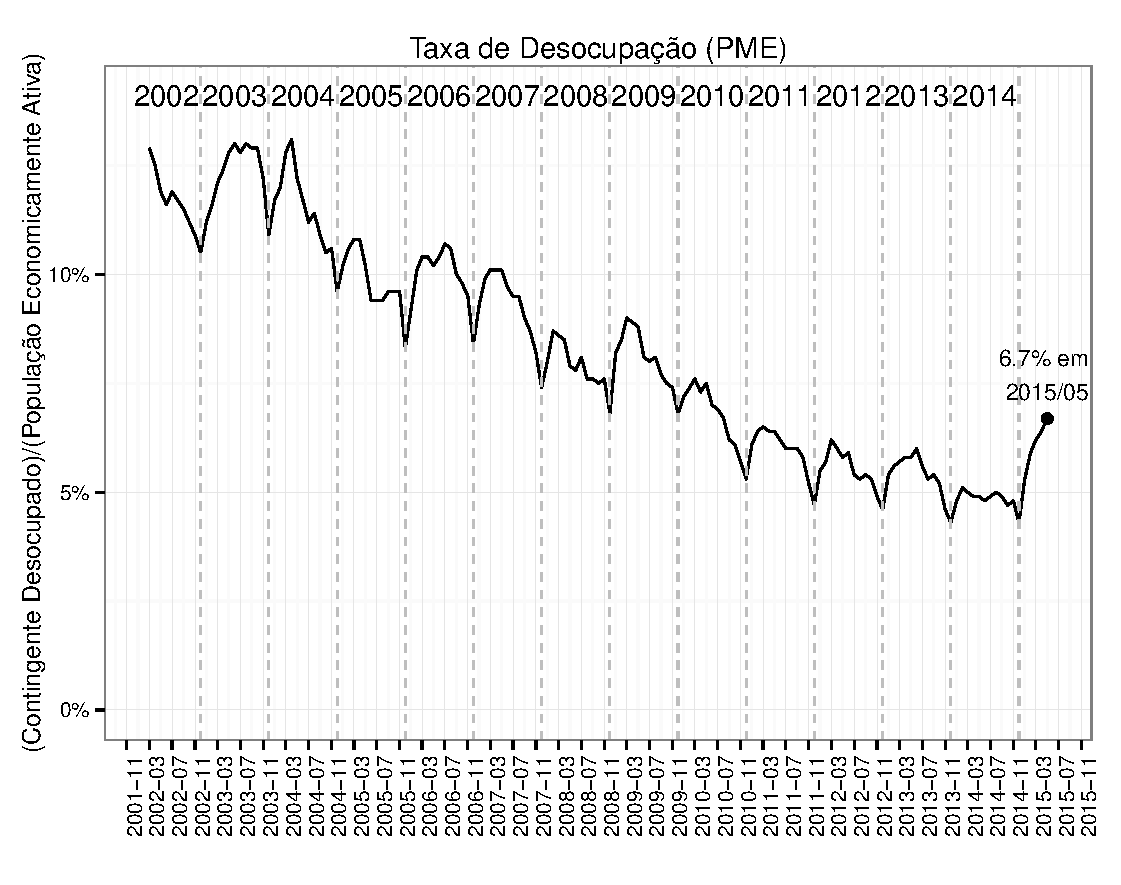
\includegraphics{Desemprego.pdf}
  \end{minipage}
\end{figure}

O IBGE classifica como pessoas desempregadas ou desocupadas aquelas que não estavam trabalhando, estavam disponíveis para trabalhar e tomaram alguma providência efetiva para conseguir trabalho nos trinta dias anteriores à semana em que responderam à pesquisa.

Teoricamente é a parte da população econômica ativa, portanto em idade adulta e em condições saudáveis para exercer alguma atividade na sociedade, e que infelizmente por circunstâncias devidas, não está podendo realizar sua função social.

Para as pesquisas realizadas entre 1983 e 2002, o IBGE considerava população em idade ativa (PIA), aqueles maiores de quinze anos de idade. De acordo com a nova metodologia do instituto, fazem parte da população em idade ativa os maiores de dez anos de idade. Na definição de população empregada ou ocupada, o instituto considerava o limite mínimo de 15 horas por semana para o trabalho não-remunerado, enquanto a nova pesquisa inclui aqueles que trabalharam pelo menos uma hora na semana.

\textbf{Fonte:} http://pt.wikipedia.org/wiki/Taxa\_de\_desemprego\_no\_Brasil

\pagebreak

\end{document}
